\section{A Customized Programming Environment}
\label{sec:environment}


The features that influence the experience of the learning programmer are not limited to the programming language she uses. 
The \emph{tools} through with the code is written, analyzed and evaluated have a paramount relevance for this experience, and therefore for the success of the programming courses.

Beginner programmers are likely to require more guidance and make more mistakes than experienced programmers.
Also, the kind of support required by experienced programmer from her development environment is different from that required by a beginner, \eg an experienced programmer might select her programming environment thinking on increasing productivity.
One very important feature a beginner requires from her programming environment is \emph{discoverability}, \ie the tools should help discover possible paths of action and gently provide feedback when the student makes a mistake, helping her to understand what was wrong and how to fix her program.
Finally, all programmers require tools that help them understand, navigate and explore their programs.

\medskip 

We decided to embed the Wollok language in an integrated programming environment, whose features are designed having in mind the specific needs of novice programmers.
In our view. the tools provided by the environment are a fundamental part of the Wollok proposal, in equal terms with the language features.

In particular, the Wollok environment provides tools focused to the following goals:
\begin{itemize}
\item To guide and ease the acual code writing.
\item To detect several of the most common mistakes done by novices, providing adequate feedback, and even to provide possible corrections when they can be computed.
\item Navigate an give different perspectives of the defined objects and classes.
\item Organize the code that is produced along the course.
\item Test and experiment with objects, both those provided by the student and those provided by Wollok.
\end{itemize}

We remark that several of the tools that the Wollok environment provides are common, in exact or approximate form, to those provided by mainstream industrial IDEs like e.g. Eclipse, Visual Studio or the Idea series. In this way, we aim to make both the programming experience more appealing to the students, and the transition to later courses and work environments softer; while giving adequate support to the learning process through the same tools.

\subsection{Basic guidance for writing code}
% To guide and ease the acual code writing
We have noticed that the first barrier for novices is the strictness of a programming language syntax. Frequently initial students find annoying that their program will not execute if they forget a closing brace or mispell a keyword or a variable name, in many cases even a case error stops execution or produces unexpected results.
Syntax highlighting is very helpful by providing a very fast visual feedback about a mispelled keyword.
Also, like many modern code editors, the Wollok IDE automatically creates a matching closing symbol each time the programmer types a parenthesis, square bracket or brace. 
Also the IDE helps correctly indenting the code inside code portions enclosed in braces or square brackets, which both helps avoiding frustrating syntax problems and starts to induce best practices about code organization.

Other approaches have addressed this problem using block-based or visual programming tools \np{Cita a alguno}. 
While we value those ideas, we think that mainstream programming is and will continue to be text-based, therefore, non-textual programming can be useful for younger students, but at universitary level it is better to provide tools that help dealing with syntax problems rather than continue circumventing them.

At a bigger scale, Wollok admits the definition of several objects and/or classes in the same file. 
This allows the teacher to go deeper in the initial examples in playing with several objects and polymorphism, without requiring the students to struggle with imports and packages.
These concepts will arise later in the course, when students' programs increase their complexity to a level that demands for modularization (\cf \ref{sec:modularization}).
\np{¿Esto no es una característica del lenguaje?}

The Wollok IDE also has integrated a powerful \emph{code analyser} that enables for \emph{content assistance}\np{¿Está bien este nombre?}, 
\ie in certain contexts, the IDE can autocomplete an identifier name, or provide a list of possible completions if there are many (\cf Fig. \ref{fig:codeCompletion}).
This is available for all types of variables and constants and messages sent to \code{self}, \code{super} or any WKO\footnote{Current work in progress includes a type inference system that once completed should allow to add content asistance for any message send}. 
 
\begin{figure}[ht]
 \centering
 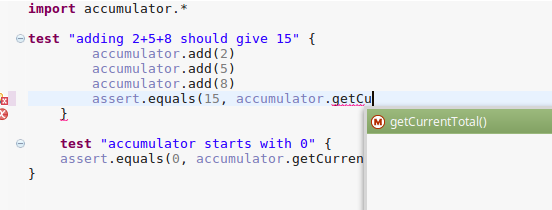
\includegraphics[scale=0.45]{images/codeCompletion.png}
 \caption{\small A list of suggestions from the Wollok IDE content assistance.}
 \label{fig:codeCompletion}
\end{figure}

\subsection{Detect mistakes and help fixing them}
\label{sec:detectMistakes}
Another dimension of the programming environment is helping the programmer to recover from his mistakes. 

First, we aim for \emph{static error detection} whenever possible, because it provides faster feedback than runtime checks.
Some errors can be even reported as the programmer is typing.
On the other hand, runtime checks are not only slower but also open to be skipped in some program executions.

Second, error reporting should provide with clear messages, explained in the same terms in which the teacher talks to the students. 
Also, inline error reports, \eg underlining the offending code, relieves the student from the task of mapping the detected problem with the possible cause 

Third, in some situations, the IDE can propose possible automatic fixes to the detected problems.
Figure \ref{fig:errorReporting} exemplifies these features. The mispelled identifier is underlined and if we put the mouse on the error report we get an error message and a possible fix.
In this case, the automatic fix will insert an empty method in the adecquate position.

\begin{figure}[ht]
 \centering
 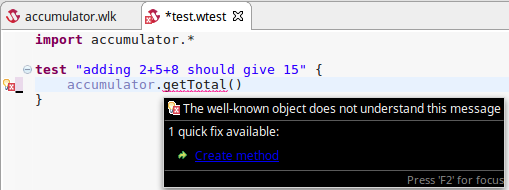
\includegraphics[scale=0.5]{images/errorReporting.png}
 \caption{\small Example of a simple error detection.}
 \label{fig:errorReporting}
\end{figure}

\medskip
Together, these characteristics are meant to empower the student to explore different ideas, 
providing positive feedback in case he makes a mistake.

While this does not replace the more personalized feedback a teacher can provide, in several situations a sensitive automatic feedback can help the student not to stay stuck with simple errors waiting for a response.
This in turn allows for more exercises during the course.

Moreover, automatic detection acts as a (basic) assistant teacher, \ie some simple topics that are not crucial for the course can be left for the student to learn by herself in the interaction with the IDE.
This is specially efficient for some kind of errors that occur only for specific groups of students, \eg those with previous non-academic OO experience. 
Tackling this errors in class, would imply to show a bad solution to the rest of the students, that had otherwise not thought about it. This would be a fine strategy in an advanced course, but will confuse beginners.
Instead, we prefer let the IDE detect the mistake and show possible solutions, only for the students that effectively incurr in these kind of errors.\np{Faltaría un ejemplo.}

\medskip

%  - Error indications with adequate messages. De esto daría algunos ejemplos que nos parezca piola resaltar, no sería exhaustivo.
%  - Quick fixes.

Finally, the great majority of validations and automatic proposals, are the result of our experience in the classroom, looking at the students using the Wollok language and IDE, as well as other languages and tools we have used in the past.
Each semester, we receive reports of the teachers using Wollok which include the type of errors the students make most often, trying to improve the network of validations and proposals, in order to improve the learning experience.

%\medskip
%This validations are organized and shown in a unified way, using a dedicated section of the user interface for their display.
%All the results of the checking and the validation of the program is shown in one integrated view, it is called \emph{Problems View}, Fig. \figref{problemsview.png} shows a view of this feature. 
%
%\begin{figure}[ht]
%    \centering
%	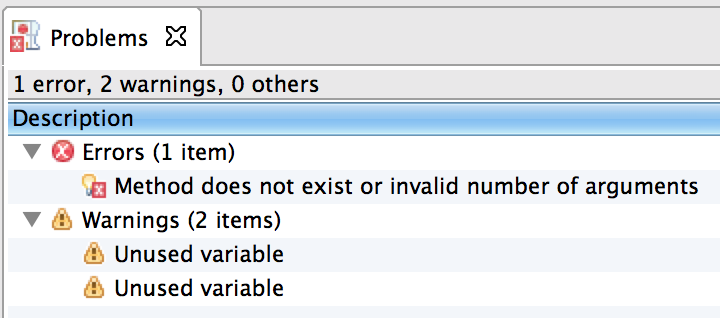
\includegraphics[scale=0.5]{images/wollok-paper-check-problemsview.png}
%    \caption{Problems View: shows the different problems detected by the IDE }
%    \label{fig:problemsview.png}
%\end{figure}
%
%Here is a list of all the validations and checks the tool supports, and a brief reason why they are useful while teaching object oriented programming:

%  \item \textbf{References resolution problems}: this errors are useful to detect and avoid references to undeclared variables and also errors in the sending of messages.
%	\begin{itemize}
%	  \item \textit{Undeclared references}: from local variables, parameters or internal fields of objects and classes.
%	  \item \textit{Undefined constructors}: checking for the number and type of the parameters.
%	  \item \textit{Messages to this}: sending messages to this is a special case, here we can check the existence of the correct method by the number and type of the arguments, even without using type inference.

\subsection{Understanding and navigating a program}
Simple \emph{code navigation} tools can significantly improve the programming experience.
For example the Wollok IDE allows to go in one click from a message send to its implementation\footnote{In the cases that is identifiable by the static analyser} and a keyboard shortcut\footnote{\code{ALT + left arrow} which is familiar to students due to its universal adoption in web browsers.} to go back to the previous location.
Fast navigation back and forth through a program allows for better understanding of the relationship between the different portions of it.
We have seen that lack of proper navigation tools might mislead the student to avoid correct modularization of their program, as they run into difficulties coping with a program that is divided in several small pieces.

Also, code visualization tools help understanding bigger programs and are as useful for beginners as they are for experienced programmers.
The Wollok IDE provides an outline view and automatic static diagrams (\cf Fig. \ref{fig:outline}).
These higher-level views of the program, allow the student to gain practice in abstracting herself of the details of some portions of a program, understanding her objects and classes as black boxes that provide some services, instead of attempting to have all of them in her head at all times, which is a necessary skill for being able to participate in a larger project.

\begin{figure}[ht]
 \centering
 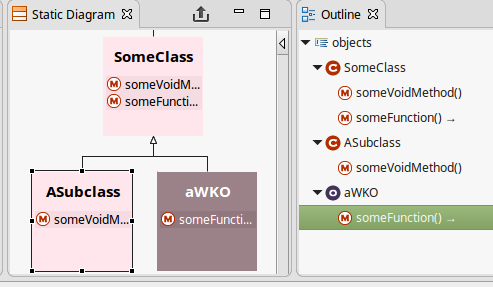
\includegraphics[scale=0.5]{images/outline.png}
 \caption{\small Example of a simple error detection.}
 \label{fig:outline}
\end{figure}

% No puse nada de:
% - Ctrl-O, es medio difícil de explicar, no sé.
% - Tampoco sé bien bien qué decir del Ctrl-E
% - Destacar que distingue los métodos con y sin efecto, si bien esto es un feature interesante, creo que es medio descolgado en este punto o habría que hablar más largo sobre por qué esa diferenciación que no está en ningún lado, creo.

\subsection{Encouraging best programming practices}
In our opinion, good practics should be taught from the very beginning of programming curricula. This claim is independent of the recurrent debate about rules and conventions. 
Our experience shows that it is unlikely that novice programmers appreciate the advantages of e.g. good variable names or correct code indentation, these being attributes that are more easily appreciated on larger programs.
Therefore, we have to actively enforce them, and have them get used to writing and reading good quality code.

Several features of the language and code editor aim to promote, or enforce, good programming practices.
For example, it compels the programmer to a predefined order inside a class definition, \ie grouping all variables and constants in the first place, then constructors and finally methods. 
Also it establishes some basic rules about naming and restricts the usage of global variables.
We also mention that autocompletion of braces and square brackets eases the adoption of adequate indentation.

Moreover, some bad programming habits are detected by the error detection of the IDE. 
As an example, Fig. \figref{check-unusedVariable.png} shows an example of an unused variable error.
Unused, \emph{dead code} tends to appear after a refactoring or after trying different solutions to a problem. 
Quick detection of this kind of errors will help the student to identify the bad practice and train her avoiding its appearance.


\commented{
A major part of the IDE is devoted to enforce good programming practices, which we consider as a main topic in a programming learning course.
For example, it compels the programmer to a predefined order inside a class definition, \ie grouping all variables and constants in the first place, then constructors and finally methods. 
Also it establishes some basic rules about naming and restricts the usage of global variables.

While the specific rules could be debated forever, and independently of the conventions chosen,
we think that good programming practices have to be taught from the very beginning.
In their first programs, students might not be able to appreciate the advantages of good variable names or correct code indentation, these are attributes that are more easily appreciated on larger programs.
Therefore, we have to actively enforce them, and have them get used to writing and reading good quality code.
We do not want them to acquire bad programming practices that will be difficult to \emph{unlearn} later.

As an example, Fig. \figref{check-unusedVariable.png} shows an example of an unused variable error.
Unused, \emph{dead code} tends to appear after a refactoring or after trying different solutions to a problem. 
Quick detection of this kind of errors will help the student to identify the bad practice and train her avoiding its appearance.
}

\begin{figure}[ht]
    \centering
	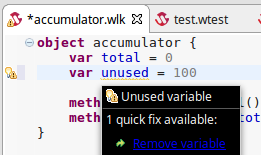
\includegraphics[scale=0.5]{images/wollok-paper-check-unusedVariable.png}
    \caption{Detection of unused variables}
    \label{fig:check-unusedVariable}
\end{figure}

\medskip
At a higher level, the Wollok IDE is designed to help the students to put in order the code they produce along the course. 
Source files are organized in \emph{projects}, that have a predefined directory structure including both files for class/object definitions and tests.
The generated file structure is adequate to the use of a source code repository such as GIT or SVN, that improves collaboration in group assignments and serves as communication tool with teachers.
%Frequently this is also accompanied by a source code repository such as GIT or SVN, which not only helps organization but also improves collaboration in group assignments and serves as communication tool with the teacher.

These features the frequent difficulties novice programmers find to organize their source files, and inparticular, to coordinate work in group assignments.
We note to this respect that it is ordinary to see members of a work group share code by sending \emph{zips} by e-mail between each other.
The time spent trying to reconcile different versions of the program or even trying to understand which is the latest one, distracts them from learning the actual topics of the course.
Hence the benefit of providing suitable source organization tools, besides the promotion of good development practices it implies.

%We note that without adequate IDE support, the organization of source files often pose difficulties to novice programmers. In particular, the coordination of work for group assignments can be problematic. 
%For example, 
%%in the absence of adequate tools 
%it is ordinary to see members of a work group share code by sending \emph{zips} by e-mail between each other.
%The time spent trying to reconcile different versions of the program or even trying to understand which is the latest one, distracts them from learning the actual topics of the course.
%
%Without adequate guidance, a group of novices, who have yet not assimilated an autonomous organization discipline, will usually encounter difficulties structuring their code or coordinating their work.
%For example, in the absence of better tools it is ordinary to see members of a work group share code by sending \emph{zips} by e-mail between each other.
%The time spent trying to reconcile different versions of the program or even trying to understand which is the latest one, distracts them from learning the actual topics of the course.

\subsection{Tests and experiments}
As we described in Section \ref{sec:wollokLanguage}, Wollok provides, as ways to work with the defined objects and classes, the REPL and the definition of tests.

The REPL provides a simple environment for direct object manipulation; it is the first tool to interact with objects that we introduce in the course.
The programmer can just send messages to the WKOs he defines, and see how they respond. 
In some courses, we even \emph{start} on the REPL, sending messages to objects provided by the teacher.
In this way, students get familiarized with the most important concepts of the OO paradigm: \emph{object} and \emph{message}, before going into the details about how these objects have been implemented.

Moreover, the REPL also allows the programmer to define local variables, which are useful to remember intermediate results to be used in further operations, making it easy for the students to perform non-trivial object manipulations.

\medskip
As the REPL interaction grows, very soon the students themselves realize that they are doing repetitive operations there and start looking for automation;
at this moment, \emph{automatic tests} are introduced.
Fig. \ref{fig:testRunner.png} shows the test runner tool output for the test shown in Fig. \ref{fig:test}.

It is important to notice that the test requires a \emph{higher level of abstraction} than the REPL.
Now the student has to anticipate the result that some expression should yield, write explicitly both expression an expected result, and interpret a \emph{green bar} as a signal that the answer yielded was the expected, without ever seeing it.

We observe that while the REPL is available all along the course, once the students become more fluent with automated tests, they use the REPL with less frequence.
Also, we remark that by the combination of REPL and tests, we have succeeded in completely avoiding the need for undesired debugging practices, such as the inclusion of \code{println} expressions along the code.

\begin{figure}[ht]

    \centering
	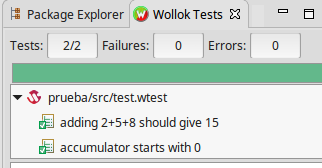
\includegraphics[scale=0.6]{images/testRunner.png}
    \caption{Test runner view after a sucessful test run.}
    \label{fig:testRunner.png}
\end{figure}

%\subsection{Type Inference}
% Type inferer
%Another distinctive characteristic of the Wollok project is the type inferer.
%We think that type inference is key to a simple programming environment.
%On one side, it allows to detect lots of common mistakes \emph{before running the program}:
%if an object does understand a message, if a wrong argument is passed, if incompatible types are mixed or even miss-spellings.
%In environments without this capability it takes more time to detect errors.
%Moreover, it is not uncommon that a type mistake produces a runtime error in a place different from where the mistake was done, producing confusion.
%
%Still, providing a type inferer for a language such as Wollok has many subtleties, which deserves an independent study \cite{passerini_nicolas_extensible_2014}.
%On one side we require it to be able to work without type annotations and at the same time provide feedback useful for an inexperienced programmer.
%On the other side, the type system is rather complex;
%for example, the presence of stand-alone objects requires the type system to handle \emph{structural types}, since a named type system would not allow them to be treated polymorphically.
%Also, we want to be able to treat polymorphically stand alone objects with class-based objects.
%\figref{check-messageSending.png} shows an error detected by the type inferer and how it shows the information to the programmer.
%Notice that the inferred type for the object \code{ufo} is a structural type: \code{fly}
%
%\begin{figure}[ht]
%    \centering
%	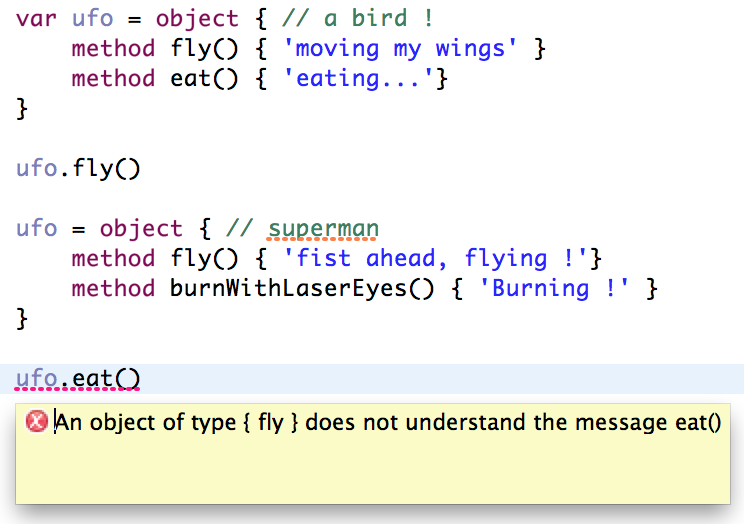
\includegraphics[scale=0.5]{images/wollok-paper-check-messageSending.png}
%    \caption{Type system in action, detecting not defined method for the message sent}
%    \label{fig:check-messageSending.png}
%\end{figure}
%
%
